\newpage
\section{LECTURE 8}

\subsection{Agenda}
\begin{itemize}
    \item Dynamic Programming
    \item Convexity
\end{itemize}

\subsection{Bellman's Principle}
\begin{itemize}
    \item Optimal control problems have an inherently sequential structure. 
    \item Past control inputs affect future states but future control inputs cannot affect past states. 
    \item Bellman's principle (i.e. The principle of optimality), states the cocnsequences of this for optimal trajectories. 
    \item Sub-trajectories of optimal trajectories have to be optimal for the appropriately defined sub-problem.
\end{itemize}

\begin{figure}
    \centering
    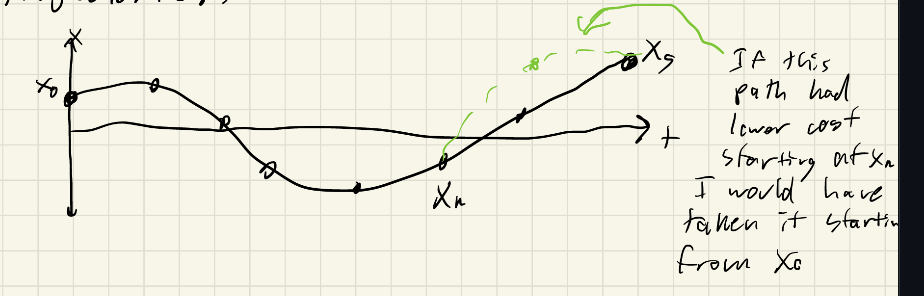
\includegraphics[width=0.4\linewidth]{L8_Images/F1.PNG}
    \caption{Bellman's Principle}
    \label{fig:l8f1}
\end{figure}

\subsection{Dynamic Programming}
\begin{itemize}
    \item Bellman's Principle suggests starting from the end of the trajectory and working backwards. 
    \item We've already seen hints of this in the Riccati equation, and in the co-state / multiplier equation from Pontryagin. 
    \item Define ``optimal cost-to-go'' a.k.a ``value function'' $V_N(x)$.
    \item Encodes the cost incurred starting from state $x$ at time $k$ if we act optimally. 
    \item For the LQR setting, we have: 
    \begin{align}
        V_N(x) = \frac{1}{2} x^T Q_N x = \frac{1}{2} x^T P_N x  
    \end{align}
    \item Now we can back up one time step, and compute $V_{N-1}(x)$:
    \begin{align}
        \min_u & \frac{1}{2} x_{N-1}^T Q x_{N-1} + \frac{1}{2} u^T R u + V_N (A_{N-1} x_{N-1} + B_{N-1} u) \\
        &= \min_u \frac{1}{2} u^T R u + \frac{1}{2} (A x_{N-1} + B_{N-1} u)^T Q_N  (A x_{N-1} + B_{N-1} u)
    \end{align}
    Since for the optimal action we have $\nabla_u $ of this cost $=0$, we have: 
\begin{align}
    u^T R_{N-1} + (A x_{N-1} + B_{N-1} u)^T Q B_{N-1} = 0 \\
    \implies u_{N-1} &= -(R_{N-1} + B_{N-1}^T Q_N B_{N-1})^{-1} B_{N-1}^T Q_N A_{N-1} x_{N-1} 
\end{align}
    We may define $K_{N-1}$ as $(R_{N-1} + B_{N-1}^T Q_N B_{N-1})^{-1} B_{N-1}^T Q_N A_{N-1}$ for convenience. 
    \item Plugging in $u=-Kx$ into our expression for $V_{N-1}(x)$, we have: 
    \begin{align}
        V_{N-1}(x) &= \frac{1}{2} x^T (Q_{N-1} + K_{N-1}^T R_{N-1} K + (A_{N-1} - B_{N-1} K_{N-1})^T Q_N (A_{N-1} - B_{N-1} K_{N-1}) ) x
    \end{align}
    We can define $P_{N-1} = (Q_{N-1} + K_{N-1}^T R_{N-1} K + (A_{N-1} - B_{N-1} K_{N-1})^T Q_N (A_{N-1} - B_{N-1} K_{N-1}) )$, such that:
    \begin{align}
        V_{N-1}(x) &= \frac{1}{2} x^T P_{N-1} x 
    \end{align}
    
    \item We now have a recursion in $K$ and $P$ that we can iterate until $k=1$. This is just the Riccati equation again. 
\end{itemize}

\subsubsection{Backward Dynamic Programming Algorithm}

\\
\noindent
\begin{algorithm}
	\caption{Backward DP Algorithm}
	\label{alg:bdp}
	\begin{algorithmic}[1]	
        \State $V_N(x) \gets l_N(x)$
        \State $K \gets N$
        \While {$K>1$} 
            \State $V_{k-1} = \min_u \big[ l(x,u) + V_k(f(x,u))\big]$ \Comment{The Bellman Equation.}
            \State $k \gets k-1$
        \EndWhile
	\end{algorithmic}
\end{algorithm}
\\

\begin{itemize}
    \item If we know $V_k(x)$, the optimal feedback policy is: 
    \begin{align}
        u_{k}(x) &= \arg\min_u \big[ l(x_k,u) + V_{k+1}(f(x_{k},u)) \big]
    \end{align}
    \item DP equations can be written equivalently in terms of action-value or $Q$ functions:
    \begin{align}
        S_k(x,u) &= l(x,u) + V_{k+1} (f(x,u)) \\
        \implies u_k(x_k) &= \arg\min_u S_k(x_k,u)
    \end{align}
    \item These are usually denoted $Q(x,u)$, be we will use $S$, since $Q$ is used in the LQR state cost as well. 
\end{itemize}

\subsubsection{The Curse}
\begin{itemize}
    \item DP is sufficient for a global optimum. 
    \item It is only tractable for simple problems, such as LQR problems or low-dimensional problems. 
    \item $V(x)$ stays quadratic for LQR problems, but becomes impossible to write down analytically for even simple non-linear problems. 
    \item Even if we could, the $\min_u S(x,u)$ will be non-convex, and possibly hard to solve on its own. 
    \item The cost of DP blows up with state dimension, due to the difficulty of representing $V(x)$. 
\end{itemize}

\subsubsection{Why do we care?}
\begin{itemize}
    \item Approximate DP, where $V(x)$, or $S(x,u)$ are reprsented with function approximators can work well. 
    \item Forms the basis of a lot of modern Reinforcement Learning. 
    \item DP generalizes to stochastic problems well, (just wrap everything in expectation operators), whereas Pontryagin's does not. 
\end{itemize}

\subsubsection{What are those Lagrange Multipliers?}
\begin{itemize}
    \item Recall Riccati derivation from QPs:
    \begin{align}
        \lambda_n &= P_n x_n \\
        P_n &= Q + A^T P_{n+1} (A-BK) \\
        &= Q + K^T R K + (A-BK)^T P_{n+1} (A-BK) \\
        V_n(x) &= \frac{1}{2} x^T P_n x \\
        \implies \lambda_n &= \nabla_x V_n(x)
    \end{align}
    \item The dynamics multipliers are the cost-to-go gradients! 
    \item Carries over to the general non-linear setting, beyond just LQR. 
\end{itemize}

\subsubsection{Example}
Remember to check out the lecture video for an example, where $\lambda_n$ from the QP matches $\nabla_x V_n(x)$ from DP. 

\subsection{Convex Model-Predictive Control}
\begin{itemize}
    \item LQR is very powerful, but often need to explicitly reason about constraints. 
    \item Often these are simple (ex. torque limits), and can be encoded as a convex set. 
    \item Constraints break the Riccati solution, but we can still solve the QP online. 
    \item Convex MPC has gotten extremely popular as computers have gotten faster. 
\end{itemize}

\subsubsection{Background: Convexity}
\begin{itemize}
    \item Convex Set: A line connecting any two points in the set is contained within the set.
    \item Standard examples:
    \begin{itemize}
        \item Linear subspaces ($Ax=b$). 
        \item Half-spaces, boxes, and polytopes ($Ax\leq b$). 
        \item Ellipsoids ($x^T P x \leq 1$).
        \item Cones ($||x_{2:n}||_2 \leq x_1$). This is called the second order cone, it's the usual ice-cream cone you're used to. 
    \end{itemize}
    \item Convex functions: A function $f(x): \matbb{R}^n \longrightarrow \mathbb{R}$ who's epigraph is a convex set. 
    \item Examples: 
    \begin{itemize}
        \item Linear $f(x) = c^T x$.
        \item Quadratic $f(x) = \frac{1}{2} x^T Q x + q^T x, \ni Q \geq 0$.
        \item Norms $f(x) = |x|$.
    \end{itemize}
    \item Convex Optimization Problem: Minimize a convex function over a convex set. 
    \item Examples:
    \begin{itemize}
        \item Linear Program (LP): Linear $f(x)$, linear $c(x)$.
        \item Quadratic Program (QP): Quadratic $f(x)$, linear $c(x)$. 
        \item Quadratically Constrained (QCQP): Quadratic $f(x)$, ellipsoid $c(x)$. 
        \item Second-order cone program (SOCP): Linear $f(x)$, cone $c(x)$. 
    \end{itemize}
    \item Convex problems don't have spurious local optima that satisfy the KKT. If you find a local KKT solution, you have the global optimum!
    \item Practically, Newton's method converges really fast and reliably (~5-10 iterations at maximum). 
    \item Can bound the solution time for real-time control.
\end{itemize}